% !TeX root = tcolorbox.tex
% include file of tcolorbox.tex (manual of the LaTeX package tcolorbox)
\clearpage
\section{Macros for Box Creation}%
\tcbset{external/prefix=external/coremacros_}%
%\subsection{Using \texttt{tcolorbox} and \texttt{\texorpdfstring{\char`\\}{\textbackslash}tcbox}}\label{subsec:macros_using}
\subsection{Using \texttt{tcolorbox} and \texttt{\textbackslash tcbox}}\label{subsec:macros_using}
\begin{docEnvironment}{tcolorbox}{\oarg{options}}
  This is the main environment to create an accentuated colored text box with
  rounded corners and, optionally, two parts. The appearance of this box
  is controlled by numerous options.
  In the most simple case the source code

\begin{dispListing}
\begin{tcolorbox}
This is a \textbf{tcolorbox}.
\end{tcolorbox}
\end{dispListing}

creates the following compiled text box:
\begin{tcolorbox}
This is a \textbf{tcolorbox}.
\end{tcolorbox}

The text content of the box can be divided
in an upper and a lower part
by the command \refCom{tcblower}. Visually, both parts are separated by a line.
For example:

\begin{dispListing}
\begin{tcolorbox}
This is another \textbf{tcolorbox}.
\tcblower
Here, you see the lower part of the box.
\end{tcolorbox}
\end{dispListing}

This code gives the following box:
\begin{tcolorbox}
This is another \textbf{tcolorbox}.
\tcblower
Here, you see the lower part of the box.
\end{tcolorbox}

The \meta{options} control the appearance and several functions of the boxes,
see \Vref{sec:optkeys} for the complete list.
A quick example is given here:

\begin{dispExample}
\begin{tcolorbox}[colback=red!5!white,colframe=red!75!black,title=My nice heading]
This is another \textbf{tcolorbox}.
\tcblower
Here, you see the lower part of the box.
\end{tcolorbox}
\end{dispExample}
\end{docEnvironment}


\begin{docCommand}{tcblower}{}
  Used inside \refEnv{tcolorbox} to separate the upper box part from
  the optional lower box part. The upper and the lower part are treated
  as separate functional units. If you only want to draw a line, see
  \refCom{tcbline}.
\end{docCommand}


\clearpage
\begin{docCommand}{tcbset}{\marg{options}}
  Sets options for every following \refEnv{tcolorbox} inside the current \TeX\ group.
  By default, this does not apply to nested boxes, see \Vref{subsec:everybox}.\par
  For example, the colors of the boxes may be defined for the whole document by this:
\begin{dispListing}
\tcbset{colback=red!5!white,colframe=red!75!black}
\end{dispListing}
\end{docCommand}


\begin{docCommand}{tcbsetforeverylayer}{\marg{options}}
  Sets options for every following \refEnv{tcolorbox} inside the current \TeX\ group.
  In contrast to \refCom{tcbset}, this does also
  apply to nested boxes, see \Vref{subsec:everybox}.
  Technically, the \meta{options} are appended to the default values for every
  tcolorbox which are applied by \refKey{/tcb/reset}.\par
  You should not use this macro, if you are not completely sure that you
  want to have the \meta{options} also for boxes in boxes (in boxes in boxes \ldots).
\begin{dispExample}
\tcbset{colback=green!10!white}
\tcbsetforeverylayer{colframe=red!75!black}

\begin{tcolorbox}[title=All options for this box]
  This is a tcolorbox.\par\medskip
  \begin{tcolorbox}[title=Nested box]
    Note that this nested box has a red frame but no green background.
  \end{tcolorbox}
\end{tcolorbox}
\bigskip

\begin{tcolorbox}[reset]
  Options given with |\tcbsetforeverylayer| survive a |reset|.
\end{tcolorbox}
\end{dispExample}
\end{docCommand}


\clearpage
\begin{docCommand}{tcbox}{\oarg{options}\marg{box content}}
  Creates a colored box which is fitted to the width of the given
  \meta{box content}. In principle, most \meta{options} for a \refEnv{tcolorbox}
  can be used for |\tcbox| with some restrictions. A |\tcbox| cannot have
  a lower part and cannot be broken.

\begin{dispExample}
\tcbset{colframe=blue!50!black,colback=white,colupper=red!50!black,
        fonttitle=\bfseries,nobeforeafter,center title}

Text \tcbox[tcbox raise base]{Hello World}\hfill
%
\tcbox[left=0mm,right=0mm,top=0mm,bottom=0mm,boxsep=0mm,
  toptitle=0.5mm,bottomtitle=0.5mm,title=My table]{%
  \arrayrulecolor{blue!50!black}\renewcommand{\arraystretch}{1.2}%
  \begin{tabular}{r|c|l}
  One   & Two    & Three \\\hline\hline
  Men   & Mice   & Lions \\\hline
  Upper & Middle & Lower
  \end{tabular}}\hfill
%
\tcbox[colback=blue!85!black,
  left=0mm,right=0mm,top=0mm,bottom=0mm,boxsep=1mm,arc=0mm,boxrule=0.5pt,
  title=My picture]{%
  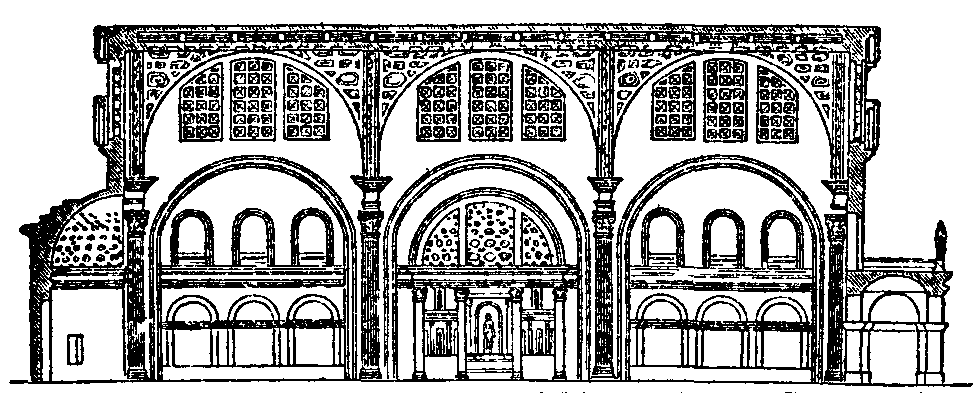
\includegraphics[width=5cm]{Basilica_5.png}}
\end{dispExample}

\begin{dispExample}
\tcbset{colframe=blue!50!black,colback=white,colupper=red!50!black,
        fonttitle=\bfseries,center title}

% Fixed width box
\begin{tcolorbox}Hello\\World!\end{tcolorbox}

% Fitted width box (like hbox or makebox)
\tcbox{Hello\\World!}

% Fitted width box (using a TikZ node)
\tcbox[tikznode]{Hello\\World!}
\end{dispExample}

\end{docCommand}


\clearpage

\begin{docCommand}{tcboxverb}{\oarg{options}\marg{verbatim box content}}
  Creates a colored box based on \refCom{tcbox} which is fitted to the width of the given
  \meta{verbatim box content}.
  The underlying \refCom{tcbox} is styled with
  \refKey{/tcb/verbatim} plus the given \meta{options}.
  The difference to \refCom{tcbox} is that the \meta{verbatim box content} is
  interpreted \textit{verbatim}. Therefore, |\tcboxverb| acts similar to |\verb|.

\begin{dispExample}
\tcboxverb{\LaTeX}, \tcboxverb[colback=blue!10!white,colupper=blue]{\LaTeX},
\tcboxverb[blank,fuzzy halo]{\LaTeX}, \tcboxverb[beamer]{\LaTeX},
\tcboxverb[enhanced,skin=enhancedmiddle jigsaw,colframe=red]{\LaTeX}.
\end{dispExample}
\end{docCommand}

\clearpage
\subsection{Producing \texttt{tcolorbox} Environments and Commands}\label{subsec:macros_tcolorbox}

\begin{docCommand}{newtcolorbox}{\oarg{init options}\marg{name}\oarg{number}\oarg{default}\marg{options}}
  Creates a new environment \meta{name} based on \refEnv{tcolorbox}.
  Basically, |\newtcolorbox| operates like |\newenvironment|. This means,
  the new environment \meta{name} optionally takes \meta{number} arguments, where
  \meta{default} is the default value for the optional first argument.
  The \meta{options} are given to the underlying |tcolorbox|.
  Note that \refKey{/tcb/savedelimiter} is set to the given \meta{name}
  automatically.
  The \meta{init options} allow setting up automatic numbering,
  see Section \ref{sec:initkeys} from page \pageref{sec:initkeys}.
\begin{dispExample*}{sbs,lefthand ratio=0.6}
\newtcolorbox{mybox}{colback=red!5!white,
  colframe=red!75!black}

\begin{mybox}
This is my own box.
\end{mybox}
\end{dispExample*}

\begin{dispExample*}{sbs,lefthand ratio=0.6}
\newtcolorbox{mybox}[1]{colback=red!5!white,
  colframe=red!75!black,fonttitle=\bfseries,
  title={#1}}

\begin{mybox}{Hello there}
This is my own box with a mandatory title.
\end{mybox}
\end{dispExample*}

\begin{dispExample*}{sbs,lefthand ratio=0.6}
\newtcolorbox{mybox}[2][]{colback=red!5!white,
  colframe=red!75!black,fonttitle=\bfseries,
  colbacktitle=red!85!black,enhanced,
attach boxed title to top center={yshift=-2mm},
  title={#2},#1}

\begin{mybox}[colback=yellow]{Hello there}
This is my own box with a mandatory title
and options.
\end{mybox}
\end{dispExample*}

\inputpreamblelisting{A}

\begin{dispExample*}{sbs,lefthand ratio=0.6}
\begin{pabox}[colback=yellow]{Hello there}
This is my own box with a mandatory
numbered title and options.
\end{pabox}
\end{dispExample*}
\end{docCommand}


\begin{docCommand}{renewtcolorbox}{\oarg{init options}\marg{name}\oarg{number}\oarg{default}\marg{options}}
  Operates like \refCom{newtcolorbox}, but based on |\renewenvironment| instead of |\newenvironment|.
  An existing environment is redefined.
\end{docCommand}


\clearpage

\begin{docCommand}{NewTColorBox}{\oarg{init options}\marg{name}\marg{specification}\marg{options}}
  Creates a new environment \meta{name} based on \refEnv{tcolorbox}.\\
  Basically, \refCom{NewTColorBox} operates like |\NewDocumentEnvironment|. This means,
  the new environment \meta{name} is constructed with the
  given \LaTeX3 argument \meta{specification} following \cite{latexproject:usrguide}.
  An error is issued if an environment with \meta{name} has already been defined.
  The \meta{options} are given to the underlying \refEnv{tcolorbox}.\\
  Note that \refKey{/tcb/savedelimiter} is set to the given \meta{name}
  automatically.\\
  The \meta{init options} allow setting up automatic numbering,
  see Section \ref{sec:initkeys} from page \pageref{sec:initkeys}.

\begin{dispExample}
% counter from previous example
\NewTColorBox[use counter from=pabox]{mybox}{ O{red} m d"" !O{} }
  {enhanced,colframe=#1!75!black,colback=#1!5!white,
   fonttitle=\bfseries,title={\thetcbcounter~#2},
   IfValueT={#3}{watermark text={#3}},#4}

\begin{mybox}{My title}
This is a tcolorbox.
\end{mybox}

\begin{mybox}[blue]{My title}
This is a tcolorbox.
\end{mybox}

\begin{mybox}[green]{My title}"My Watermark"
This is a tcolorbox.
\end{mybox}

\begin{mybox}[yellow]{My title}[colbacktitle=yellow!50!white,coltitle=black]
This is a tcolorbox.
\end{mybox}

\begin{mybox}[purple]{My title}"All together"[coltitle=yellow]
This is a tcolorbox.
\end{mybox}
\end{dispExample}
\end{docCommand}

\clearpage
\begin{docCommand}{RenewTColorBox}{\oarg{init options}\marg{name}\marg{specification}\marg{options}}
  Operates like \refCom{NewTColorBox}, but based on |\RenewDocumentEnvironment| instead of |\NewDocumentEnvironment|.
  An existing environment is redefined.
\end{docCommand}

\begin{docCommand}{ProvideTColorBox}{\oarg{init options}\marg{name}\marg{specification}\marg{options}}
  Operates like \refCom{NewTColorBox}, but based on |\ProvideDocumentEnvironment| instead of |\NewDocumentEnvironment|.
  The environment \meta{name} is only created if it is not already defined.
\end{docCommand}

\begin{docCommand}{DeclareTColorBox}{\oarg{init options}\marg{name}\marg{specification}\marg{options}}
  Operates like \refCom{NewTColorBox}, but based on |\DeclareDocumentEnvironment| instead of |\NewDocumentEnvironment|.
  The new environment is always created, irrespective of an already existing
  environment with the same name.
\end{docCommand}


\clearpage

\begin{docCommand}{NewTotalTColorBox}{\oarg{init options}\brackets{\texttt{\textbackslash}\meta{name}}\marg{specification}\marg{options}\marg{content}}
  Creates a new command \texttt{\textbackslash}\meta{name} based on \refEnv{tcolorbox}.
  In contrast to \refCom{NewTColorBox}, also the \meta{content} of the |tcolorbox| is specified.\\
  Basically, \refCom{NewTotalTColorBox} operates like |\NewDocumentCommand|. This means,
  the new command \texttt{\textbackslash}\meta{name} is constructed with the given
  \LaTeX3 argument \meta{specification} following \cite{latexproject:usrguide}.
  An error is issued if \texttt{\textbackslash}\meta{name} has already been defined.
  The \meta{options} are given to the underlying \refEnv{tcolorbox} which is filled with
  the specified \meta{content}.\\
  Note that \refKey{/tcb/savedelimiter} is set to the given \meta{name}
  automatically.
  Also note that \refKey{/tcb/saveto}, \refKey{/tcb/savelowerto},
  and \refKey{/tcb/redirectlowerto}
  cannot be used with \refCom{NewTotalTColorBox} and friends.\\
  The \meta{init options} allow setting up automatic numbering,
  see Section \ref{sec:initkeys} from page \pageref{sec:initkeys}.

\begin{dispExample}
\NewTotalTColorBox{\diabox}{ O{} v  m }
  { bicolor,nobeforeafter,equal height group=diabox,width=5.7cm,
    fonttitle=\bfseries\ttfamily,adjusted title={#2},center title,
    colframe=blue!20!black,leftupper=0mm,rightupper=0mm,colback=black!75!white,#1}
  { \tikz\path[fill zoom image={#2}] (0,0) rectangle (\linewidth,4cm);%
    \tcblower#3}

\diabox{blueshade.png}{Created with |GIMP|.\\\url{http://www.gimp.org}}
\diabox{goldshade.png}{Created with |GIMP|.\\\url{http://www.gimp.org}}
\end{dispExample}
\end{docCommand}

\begin{docCommand}{RenewTotalTColorBox}{\oarg{init options}\brackets{\texttt{\textbackslash}\meta{name}}\marg{specification}\marg{options}\marg{content}}
  Operates like \refCom{NewTotalTColorBox}, but based on |\RenewDocumentCommand| instead of |\NewDocumentCommand|.
  An existing command is redefined.
\end{docCommand}

\begin{docCommand}{ProvideTotalTColorBox}{\oarg{init options}\brackets{\texttt{\textbackslash}\meta{name}}\marg{specification}\marg{options}\marg{content}}
  Operates like \refCom{NewTotalTColorBox}, but based on |\ProvideDocumentCommand| instead of |\NewDocumentCommand|.
  The command \texttt{\textbackslash}\meta{name} is only created if it is not already defined.
\end{docCommand}

\begin{docCommand}{DeclareTotalTColorBox}{\oarg{init options}\brackets{\texttt{\textbackslash}\meta{name}}\marg{specification}\marg{options}\marg{content}}
  Operates like \refCom{NewTotalTColorBox}, but based on |\DeclareDocumentCommand| instead of |\NewDocumentCommand|.
  The new command is always created, irrespective of an already existing
  command with the same name.
\end{docCommand}


\clearpage
\subsection{Producing \texttt{\textbackslash tcbox} Commands}\label{subsec:macros_tcbox}
\enlargethispage*{10mm}

\begin{docCommand}{newtcbox}{\oarg{init options}\brackets{\texttt{\textbackslash}\meta{name}}\oarg{number}\oarg{default}\marg{options}}
  Creates a new macro \texttt{\textbackslash}\meta{name} based on \refCom{tcbox}.
  Basically, |\newtcbox| operates like |\newcommand|.
  The new macro \texttt{\textbackslash}\meta{name} optionally takes \meta{number}$+1$ arguments (up to 10), where
  \meta{default} is the default value for the optional first argument.
  Additional to the \meta{number} arguments, there is an
  automatic last (mandatory) argument of \texttt{\textbackslash}\meta{name} which takes the box content
  The \meta{options} are given to the underlying |tcbox|.
  The \meta{init options} allow setting up automatic numbering,
  see Section \ref{sec:initkeys} from page \pageref{sec:initkeys}.
\begin{dispExample*}{sbs,lefthand ratio=0.6}
\newtcbox{\mybox}{colback=red!5!white,
  colframe=red!75!black}

\mybox{This is my own box.}
\end{dispExample*}

\begin{dispExample*}{sbs,lefthand ratio=0.6}
\newtcbox{\mybox}[1]{colback=red!5!white,
  colframe=red!75!black,fonttitle=\bfseries,
  title={#1}}

\mybox{Hello there}{This is my own box.}
\end{dispExample*}

\begin{dispExample*}{sbs,lefthand ratio=0.6}
\newtcbox{\mybox}[2][]{colback=red!5!white,
  colframe=red!75!black,fonttitle=\bfseries,
  title={#2},#1}

\mybox[colback=yellow]{Hello there}%
  {This is my own box.}
\end{dispExample*}

\inputpreamblelisting{B}

\begin{dispExample*}{sbs,lefthand ratio=0.6}
\pbbox[colback=yellow]{Hello there}%
  {This is my own box.}
\end{dispExample*}

\begin{dispExample}
\newtcbox{\mybox}[1][red]{on line,
  arc=0pt,outer arc=0pt,colback=#1!10!white,colframe=#1!50!black,
  boxsep=0pt,left=1pt,right=1pt,top=2pt,bottom=2pt,
  boxrule=0pt,bottomrule=1pt,toprule=1pt}
\newtcbox{\xmybox}[1][red]{on line,
  arc=7pt,colback=#1!10!white,colframe=#1!50!black,
  before upper={\rule[-3pt]{0pt}{10pt}},boxrule=1pt,
  boxsep=0pt,left=6pt,right=6pt,top=2pt,bottom=2pt}

The \mybox[green]{quick} brown \mybox{fox} \mybox[blue]{jumps} over the
\mybox[green]{lazy} \mybox{dog}.\par
The \xmybox[green]{quick} brown \xmybox{fox} \xmybox[blue]{jumps} over the
\xmybox[green]{lazy} \xmybox{dog}.
\end{dispExample}
\end{docCommand}


\clearpage
\begin{docCommand}{renewtcbox}{\oarg{init options}\brackets{\texttt{\textbackslash}\rmfamily\meta{name}}\oarg{number}\oarg{default}\marg{options}}
  Operates like \refCom{newtcbox}, but based on |\renewcommand| instead of |\newcommand|.
  An existing macro is redefined.
\end{docCommand}


\begin{docCommand}{NewTCBox}{\oarg{init options}\brackets{\texttt{\textbackslash}\meta{name}}\marg{specification}\marg{options}}
  Creates a new command \texttt{\textbackslash}\meta{name} based on \refCom{tcbox}.
  Basically, \refCom{NewTCBox} operates like |\NewDocumentCommand|. This means,
  the new command \texttt{\textbackslash}\meta{name} is constructed with the given
  \LaTeX3 argument \meta{specification} following \cite{latexproject:usrguide}.
  Additional to the argument \meta{specification}, there is an
  automatic last (mandatory) argument of \texttt{\textbackslash}\meta{name} which takes the box content.
  Therefore, \texttt{\textbackslash}\meta{name} may have up to 10 arguments in sum.
  An error is issued if \texttt{\textbackslash}\meta{name} has already been defined.
  The \meta{options} are given to the underlying \refCom{tcbox}.\\
  Note that \refKey{/tcb/savedelimiter} is set to the given \meta{name}
  automatically.\\
  The \meta{init options} allow setting up automatic numbering,
  see Section \ref{sec:initkeys} from page \pageref{sec:initkeys}.

\begin{dispExample}
% counter from previous example
\NewTCBox[use counter from=pabox]{\mybox}{ s m s }
{ nobeforeafter,colback=red!5!white,colframe=red!75!black,
  title={#2 (Box \thetcbcounter)},fonttitle=\bfseries,
  IfBooleanT={#1}{enhanced,drop shadow},
  IfBooleanT={#3}{colbacktitle=red!50!white} }

\mybox{Bird}{This is my first box.}
  \hfill
\mybox*{Tree}{This is my second box.}
  \par\bigskip
\mybox{Bike}*{This is my third box.}
  \hfill
\mybox*{City}*{This is my fourth box.}
\end{dispExample}
\end{docCommand}


\begin{docCommand}{RenewTCBox}{\oarg{init options}\brackets{\texttt{\textbackslash}\meta{name}}\marg{specification}\marg{options}}
  Operates like \refCom{NewTCBox}, but based on |\RenewDocumentCommand| instead of |\NewDocumentCommand|.
  An existing command is redefined.
\end{docCommand}

\begin{docCommand}{ProvideTCBox}{\oarg{init options}\brackets{\texttt{\textbackslash}\meta{name}}\marg{specification}\marg{options}}
  Operates like \refCom{NewTCBox}, but based on |\ProvideDocumentCommand| instead of |\NewDocumentCommand|.
  The command \texttt{\textbackslash}\meta{name} is only created if it is not already defined.
\end{docCommand}

\begin{docCommand}{DeclareTCBox}{\oarg{init options}\brackets{\texttt{\textbackslash}\meta{name}}\marg{specification}\marg{options}}
  Operates like \refCom{NewTCBox}, but based on |\DeclareDocumentCommand| instead of |\NewDocumentCommand|.
  The new command is always created, irrespective of an already existing
  command with the same name.
\end{docCommand}


\clearpage

\begin{docCommand}{NewTotalTCBox}{\oarg{init options}\brackets{\texttt{\textbackslash}\meta{name}}\marg{specification}\marg{options}\marg{content}}
  Creates a new command \texttt{\textbackslash}\meta{name} based on \refCom{tcbox}.
  In contrast to \refCom{NewTCBox}, also the \meta{content} of the |tcbox| is specified.\\
  Basically, \refCom{NewTotalTCBox} operates like |\NewDocumentCommand|. This means,
  the new command \texttt{\textbackslash}\meta{name} is constructed with the
  given \LaTeX3 argument \meta{specification} following \cite{latexproject:usrguide}.
  An error is issued if \texttt{\textbackslash}\meta{name} has already been defined.
  The \meta{options} are given to the underlying \refCom{tcbox} which is filled with
  the specified \meta{content}.\\
  Note that \refKey{/tcb/savedelimiter} is set to the given \meta{name}
  automatically.\\
  The \meta{init options} allow setting up automatic numbering,
  see Section \ref{sec:initkeys} from page \pageref{sec:initkeys}.

\begin{dispExample}
\NewTotalTCBox{\myverb}{ O{red} v !O{} }
{ fontupper=\ttfamily,nobeforeafter,tcbox raise base,arc=0pt,outer arc=0pt,
  top=0pt,bottom=0pt,left=0mm,right=0mm,
  leftrule=0pt,rightrule=0pt,toprule=0.3mm,bottomrule=0.3mm,boxsep=0.5mm,
  colback=#1!10!white,colframe=#1!50!black,#3}{#2}

To set a word \textbf{bold} in \myverb{\LaTeX}, use
\myverb[green]{\textbf{bold}}. Alternatively, write
\myverb[yellow]{{\bfseries bold}}.
In \myverb[blue]{\LaTeX}[enhanced,fuzzy halo], other font settings are
done in the same way, e.\,g. \myverb{\textit}, \myverb{\itshape}\\
or \myverb[brown]{\texttt}, \myverb[brown]{\ttfamily}.
\end{dispExample}

The next example uses |\lstinline| from the \refPkg{listings} package to
typeset the verbatim content.

\begin{dispExample}
% \usepackage{listings} or \tcbuselibrary{listings}
\NewTotalTCBox{\commandbox}{ s v }
{verbatim,colupper=white,colback=black!75!white,colframe=black}
{\IfBooleanT{#1}{\textcolor{red}{\ttfamily\bfseries > }}%
  \lstinline[language=command.com,keywordstyle=\color{blue!35!white}\bfseries]^#2^}

\commandbox*{cd "My Documents"} changes to directory \commandbox{My Documents}.

\commandbox*{dir /A} lists the directory content.

\commandbox*{copy example.txt d:\target} copies \commandbox{example.txt} to
  \commandbox{d:\target}.
\end{dispExample}
\end{docCommand}

\clearpage

\begin{docCommand}{RenewTotalTCBox}{\oarg{init options}\brackets{\texttt{\textbackslash}\meta{name}}\marg{specification}\marg{options}\marg{content}}
  Operates like \refCom{NewTotalTCBox}, but based on |\RenewDocumentCommand| instead of |\NewDocumentCommand|.
  An existing command is redefined.
\end{docCommand}

\begin{docCommand}{ProvideTotalTCBox}{\oarg{init options}\brackets{\texttt{\textbackslash}\meta{name}}\marg{specification}\marg{options}\marg{content}}
  Operates like \refCom{NewTotalTCBox}, but based on |\ProvideDocumentCommand| instead of |\NewDocumentCommand|.
  The command \texttt{\textbackslash}\meta{name} is only created if it is not already defined.
\end{docCommand}

\begin{docCommand}{DeclareTotalTCBox}{\oarg{init options}\brackets{\texttt{\textbackslash}\meta{name}}\marg{specification}\marg{options}\marg{content}}
  Operates like \refCom{NewTotalTCBox}, but based on |\NewDocumentCommand| instead of |\DeclareDocumentCommand|.
  The new command is always created, irrespective of an already existing
  command with the same name.
\end{docCommand}



%\clearpage
\subsection{Redefining other Environments (Wrapping with \texttt{tcolorbox})}\label{subsec:macros_refine}

\begin{docCommand}[doc new=2014-10-20]{tcolorboxenvironment}{\marg{name}\marg{options}}
  An existing environment \meta{name} is redefined to be boxed inside a
  |tcolorbox| with the given \meta{options}.
\begin{dispExample*}{sbs,lefthand ratio=0.6}
% tcbuselibrary{skins}
\newenvironment{myitemize}{%
  \begin{itemize}}{\end{itemize}}

\tcolorboxenvironment{myitemize}{blanker,
  before skip=6pt,after skip=6pt,
  borderline west={3mm}{0pt}{red}}

Some text.
\begin{myitemize}
\item Alpha
\item Beta
\item Gamma
\end{myitemize}
More text.
\end{dispExample*}

\medskip
See further examples in \Vref{subsec:theorems_other}.
\end{docCommand}

